% Nguồn SGK Toán 9 Tập hai — Bài 22, trang 32--37:
% https://cdn3.olm.vn/upload/thuvienso/4491669493-page-32-1771844545274.png
% https://cdn3.olm.vn/upload/thuvienso/4491669493-page-33-1771844545599.png
% https://cdn3.olm.vn/upload/thuvienso/4491669493-page-34-1771844545908.png
% https://cdn3.olm.vn/upload/thuvienso/4491669493-page-35-1771844546233.png
% https://cdn3.olm.vn/upload/thuvienso/4491669493-page-36-1771844546534.png
% https://cdn3.olm.vn/upload/thuvienso/4491669493-page-37-1771844546836.png
% Nguồn SBT Toán 9 Tập hai — Bài 22, PDF trang 24--26:
% SBT TOÁN 9 TẬP 2.pdf
% SHA-256: 5ff01fd213d1adc75f9c54b4408d6a9642a4d8038e685040efef3311a196196c

\section{Bảng tần số và biểu đồ tần số}

\begin{lesson}
    \subsection{Kiến thức trọng tâm}

    Với dãy dữ liệu $x_1$, $x_2$, \ldots, $x_n$ có nhiều giá trị giống nhau thì có cách nào biểu diễn dãy dữ liệu này thuận tiện hơn không? Chúng ta sẽ tìm hiểu vấn đề này trong bài học.

    \textbf{1. BẢNG TẦN SỐ}

    \textbf{HĐ1. Tần số và bảng tần số}

    Bạn Minh muốn tìm hiểu về dự định của các bạn học sinh khối lớp 9 trong trường sau khi tốt nghiệp Trung học cơ sở. Em hãy giúp bạn Minh thực hiện khảo sát ý kiến của các bạn trong lớp mình theo mẫu phiếu bên.

    \begin{quote}
        \textbf{Dự định của bạn sau khi học xong lớp 9?}

        (Chỉ chọn một lựa chọn)

        A. Học Trung học phổ thông trong nước.

        B. Đi du học.

        C. Đi học nghề.

        D. Lựa chọn khác.
    \end{quote}

    \begin{enumerate}[label=\alph*)]
        \item Bạn Minh muốn khảo sát ý kiến của những ai? Em đã giúp bạn Minh khảo sát ý kiến của tất cả những người đó?
        \item Liệt kê dãy dữ liệu thu được và đếm số học sinh theo mỗi lựa chọn.
    \end{enumerate}

    \answerline
    \answerline

    \textbf{Nhận xét.} Dữ liệu mà bạn Minh muốn có là dữ liệu về ý kiến của tất cả học sinh khối lớp 9 trong trường. Dãy dữ liệu mà em thu được trong khảo sát trên là một phần của dữ liệu mà bạn Minh muốn có và được gọi là \textit{mẫu dữ liệu}. Số giá trị của mẫu dữ liệu được gọi là \textit{cỡ mẫu}.

    \begin{keyconcept}
        \begin{itemize}
            \item \textit{Tần số} của một giá trị là số lần xuất hiện giá trị đó trong mẫu dữ liệu.
            \item \textit{Bảng tần số} là bảng thống kê cho biết tần số của các giá trị trong mẫu dữ liệu. Bảng tần số có dạng sau:
        \end{itemize}

        \begin{center}
        \begin{tblr}{
            colspec={Q[c] Q[c] Q[c] Q[c] Q[c]},
            row{1}={font=\bfseries}
        }
            Giá trị & $x_1$ & $x_2$ & \ldots & $x_k$ \\
            Tần số & $m_1$ & $m_2$ & \ldots & $m_k$ \\
        \end{tblr}
        \end{center}

        trong đó $m_1$ là tần số của $x_1$, $m_2$ là tần số của $x_2$, \ldots, $m_k$ là tần số của $x_k$.
    \end{keyconcept}

    Lập bảng tần số cho mẫu dữ liệu thu được trong HĐ1.

    \answerline
    \answerline

    \textbf{Chú ý.} Người ta còn cho bảng tần số ở dạng cột: cột thứ nhất ghi các giá trị, cột thứ hai ghi tần số của các giá trị đó.

    \textbf{Ví dụ 1.} Để mua giày thể thao cho các bạn nam trong lớp luyện tập chuẩn bị cho giải bóng đá của trường, Huy đã thu thập cỡ giày của các bạn nam trong lớp và thu được kết quả như sau:

    \[
        40,\ 36,\ 37,\ 36,\ 40,\ 38,\ 39,\ 38,\ 37,\ 36,\ 40,\ 39,\ 36,\ 38,\ 37,\ 38,\ 38,\ 37,\ 38,\ 38,\ 38,\ 36.
    \]

    \begin{enumerate}[label=\alph*)]
        \item Bạn Huy cần mua giày các cỡ nào? Mỗi loại bao nhiêu đôi?
        \item Lập bảng tần số cho dãy dữ liệu trên. Từ bảng tần số, cho biết cỡ giày nào phù hợp với nhiều bạn nam trong lớp nhất.
    \end{enumerate}

    \textbf{Giải}

    a) Bạn Huy cần mua giày với các cỡ 36, 37, 38, 39, 40. Giày cỡ 36 cần 5 đôi; cỡ 37 cần 4 đôi; cỡ 38 cần 8 đôi; cỡ 39 cần 2 đôi; cỡ 40 cần 3 đôi.

    b) Bảng tần số:

    \begin{center}
    \begin{tblr}{
        colspec={Q[l] *{5}{Q[c]}},
        row{1}={font=\bfseries}
    }
        Cỡ giày & 36 & 37 & 38 & 39 & 40 \\
        Tần số & 5 & 4 & 8 & 2 & 3 \\
    \end{tblr}
    \end{center}

    Giày cỡ 38 phù hợp với nhiều bạn nam trong lớp nhất.

    \textbf{Luyện tập 1.} Bảng sau đây ghi lại tên các bạn đạt điểm tốt vào các ngày trong tuần của lớp 9E, mỗi điểm tốt ghi tên một lần.

    \begin{center}
    \begin{tblr}{
        width=\linewidth,
        colspec={X[1.6,c,m] *{5}{X[c,m]}},
        row{1}={font=\bfseries},
        cells={valign=m}
    }
        Ngày & Thứ Hai & Thứ Ba & Thứ Tư & Thứ Năm & Thứ Sáu \\
        Tên bạn đạt điểm tốt & {Bình\\Nam} & {Tuấn\\Thảo} & Bình & {Yến\\Nam} & {Nam\\Thảo} \\
    \end{tblr}
    \end{center}

    \begin{enumerate}[label=\alph*)]
        \item Trong tuần những bạn nào đạt điểm tốt? Mỗi bạn đạt được mấy điểm tốt?
        \item Lập bảng tần số cho dãy dữ liệu này. Bạn nào có số lần đạt điểm tốt nhiều nhất?
    \end{enumerate}

    \answerline
    \answerline

    \textbf{Nhận xét.} Trong bảng tần số, ta chỉ liệt kê các giá trị $x_i$ khác nhau. Các giá trị $x_i$ này có thể không là số.

    Tần số của một giá trị cho biết giá trị đó xuất hiện trong mẫu dữ liệu nhiều hay ít, từ đó ta dễ dàng xác định được giá trị xuất hiện nhiều nhất, ít nhất.

    \textbf{2. BIỂU ĐỒ TẦN SỐ}

    \textbf{HĐ2. Tìm hiểu về biểu đồ tần số}

    Cho hai biểu đồ sau:

    \begin{center}
    \begin{tikzpicture}[x=0.8cm,y=0.26cm]
        \foreach \y in {0,5,10,15} {
            \draw[base200] (0,\y)--(6.4,\y);
            \node[left] at (0,\y) {\y};
        }
        \draw[->] (0,0)--(6.6,0);
        \draw[->] (0,0)--(0,16.5);
        \foreach \x/\v in {1/6,2/7,3/8,4/9,5/10} {
            \node[below] at (\x,0) {\v};
        }
        \foreach \x/\h in {1/3,2/8,3/12,4/6,5/4} {
            \fill[base700] (\x-0.25,0) rectangle (\x+0.25,\h);
            \node[above] at (\x,\h) {\h};
        }
        \node[font=\bfseries] at (3.1,18) {Kết quả kiểm tra môn Toán};
        \node[below] at (3.2,-2.2) {Điểm};
        \node[rotate=90] at (-1.15,8) {Tần số};
    \end{tikzpicture}

    \textit{Hình 7.1. Biểu đồ A}
    \end{center}

    \begin{center}
    \begin{tikzpicture}[x=0.8cm,y=0.26cm]
        \foreach \y in {0,5,10,15} {
            \draw[base200] (0,\y)--(6.4,\y);
            \node[left] at (0,\y) {\y};
        }
        \draw[->] (0,0)--(6.6,0);
        \draw[->] (0,0)--(0,16.5);
        \foreach \x/\v in {1/6,2/7,3/8,4/9,5/10} {
            \node[below] at (\x,0) {\v};
        }
        \draw[base700,thick] (1,3)--(2,8)--(3,12)--(4,6)--(5,4);
        \foreach \x/\h in {1/3,2/8,3/12,4/6,5/4} {
            \fill[base700] (\x,\h) circle (2pt);
            \node[above right] at (\x,\h) {\h};
        }
        \node[font=\bfseries] at (3.1,18) {Kết quả kiểm tra môn Toán};
        \node[below] at (3.2,-2.2) {Điểm};
        \node[rotate=90] at (-1.15,8) {Số học sinh};
    \end{tikzpicture}

    \textit{Hình 7.2. Biểu đồ B}
    \end{center}

    \begin{enumerate}[label=\alph*)]
        \item Đọc và giải thích mỗi biểu đồ trên.
        \item Hai biểu đồ trên có biểu diễn cùng một dữ liệu không? Lập bảng thống kê cho dữ liệu đó. Bảng thống kê thu được có phải là bảng tần số hay không?
    \end{enumerate}

    \answerline
    \answerline

    \begin{keyconcept}
        Biểu đồ biểu diễn bảng tần số được gọi là \textit{biểu đồ tần số}. Biểu đồ tần số thường gặp là biểu đồ tần số dạng cột (H.7.1) và biểu đồ tần số dạng đoạn thẳng (H.7.2).
    \end{keyconcept}

    Biểu đồ tần số dạng đoạn thẳng còn gọi là đa giác tần số \allowbreak(frequency polygon).

    \textbf{Nhận xét.}
    \begin{itemize}
        \item Biểu đồ tần số dạng cột chính là biểu đồ cột với trục đứng biểu diễn tần số.
        \item Để vẽ biểu đồ tần số dạng đoạn thẳng ta thực hiện theo các bước sau:
    \end{itemize}

    \textit{Bước 1.} Vẽ trục ngang để biểu diễn các giá trị trong dãy dữ liệu, vẽ trục đứng thể hiện tần số.

    \textit{Bước 2.} Với mỗi giá trị trên trục ngang và tần số tương ứng ta xác định một điểm. Nối các điểm liên tiếp với nhau.

    \textit{Bước 3.} Ghi chú giải cho các trục, các điểm và tiêu đề của biểu đồ.

    \textbf{Ví dụ 2.} Bạn Bình thống kê số anh, chị, em ruột của các bạn trong lớp và thu được bảng sau:

    \begin{center}
    \begin{tblr}{
        colspec={Q[l] *{4}{Q[c]}},
        row{1}={font=\bfseries}
    }
        Số anh, chị, em ruột & 0 & 1 & 2 & 3 \\
        Số bạn & 8 & 19 & 6 & 4 \\
    \end{tblr}
    \end{center}

    Vẽ biểu đồ tần số dạng cột và biểu đồ tần số dạng đoạn thẳng biểu diễn bảng thống kê trên.

    \textbf{Giải}

    \begin{itemize}
        \item Vẽ biểu đồ tần số dạng cột (H.7.3).
    \end{itemize}

    \begin{center}
    \begin{tikzpicture}[x=1.2cm,y=0.22cm]
        \foreach \y in {0,5,10,15,20} {
            \draw[base200] (0,\y)--(4.4,\y);
            \node[left] at (0,\y) {\y};
        }
        \draw[->] (0,0)--(4.6,0);
        \draw[->] (0,0)--(0,22);
        \foreach \x/\v in {0.6/0,1.6/1,2.6/2,3.6/3} {
            \node[below] at (\x,0) {\v};
        }
        \foreach \x/\h in {0.6/8,1.6/19,2.6/6,3.6/4} {
            \fill[base700] (\x-0.25,0) rectangle (\x+0.25,\h);
            \node[above] at (\x,\h) {\h};
        }
        \node[font=\bfseries] at (2.2,24) {Bạn có mấy anh, chị, em ruột?};
        \node[below] at (2.2,-2.5) {Số anh, chị, em ruột};
        \node[rotate=90] at (-1.1,11) {Số học sinh};
    \end{tikzpicture}

    \textit{Hình 7.3}
    \end{center}

    \begin{itemize}
        \item Vẽ biểu đồ tần số dạng đoạn thẳng.
    \end{itemize}

    \textit{Bước 1.} Vẽ các trục (H.7.4).

    \begin{center}
    \begin{tikzpicture}[x=1.2cm,y=0.22cm]
        \foreach \y in {0,5,10,15,20} {
            \draw[base200] (0,\y)--(4.4,\y);
            \node[left] at (0,\y) {\y};
        }
        \draw[->] (0,0)--(4.6,0);
        \draw[->] (0,0)--(0,22);
        \foreach \x/\v in {0.6/0,1.6/1,2.6/2,3.6/3} {
            \node[below] at (\x,0) {\v};
        }
        \draw[base700,thick] (0.6,8)--(1.6,19)--(2.6,6)--(3.6,4);
        \foreach \x/\h in {0.6/8,1.6/19,2.6/6,3.6/4} {
            \fill[base700] (\x,\h) circle (2pt);
        }
    \end{tikzpicture}

    \textit{Hình 7.4}
    \end{center}

    \textit{Bước 2.} Xác định các điểm và nối các điểm liên tiếp với nhau (H.7.4).

    \textit{Bước 3.} Ghi chú giải cho các trục, các điểm và tiêu đề của biểu đồ (H.7.5).

    \begin{center}
    \begin{tikzpicture}[x=1.2cm,y=0.22cm]
        \foreach \y in {0,5,10,15,20} {
            \draw[base200] (0,\y)--(4.4,\y);
            \node[left] at (0,\y) {\y};
        }
        \draw[->] (0,0)--(4.6,0);
        \draw[->] (0,0)--(0,22);
        \foreach \x/\v in {0.6/0,1.6/1,2.6/2,3.6/3} {
            \node[below] at (\x,0) {\v};
        }
        \draw[base700,thick] (0.6,8)--(1.6,19)--(2.6,6)--(3.6,4);
        \foreach \x/\h in {0.6/8,1.6/19,2.6/6,3.6/4} {
            \fill[base700] (\x,\h) circle (2pt);
            \node[above right] at (\x,\h) {\h};
        }
        \node[font=\bfseries] at (2.2,24) {Bạn có mấy anh, chị, em ruột?};
        \node[below] at (2.2,-2.5) {Số anh, chị, em ruột};
        \node[rotate=90] at (-1.1,11) {Số học sinh};
    \end{tikzpicture}

    \textit{Hình 7.5}
    \end{center}

    \textbf{Luyện tập 2.} Bảng tần số sau cho biết số học sinh của lớp 9D dự đoán đội bóng vô địch World Cup 2022 trước khi giải đấu bắt đầu.

    \begin{center}
    \begin{tblr}{
        colspec={Q[l] *{4}{Q[c]}},
        row{1}={font=\bfseries}
    }
        Đội bóng & Brazil & Anh & Pháp & Argentina \\
        Số bạn dự đoán & 8 & 15 & 12 & 5 \\
    \end{tblr}
    \end{center}

    Vẽ biểu đồ tần số dạng cột và biểu đồ tần số dạng đoạn thẳng biểu diễn bảng tần số trên.

    \answerline
    \answerline
    \answerline

    \textbf{Tranh luận.} Biểu đồ cột sau biểu diễn nhiệt độ trung bình tháng Sáu tại ba thành phố của Việt Nam năm 2021.

    \begin{center}
    \begin{tikzpicture}[x=1.5cm,y=0.18cm]
        \foreach \y in {0,5,10,15,20,25,30,35} {
            \draw[base200] (0,\y)--(4.5,\y);
            \node[left] at (0,\y) {\y};
        }
        \draw[->] (0,0)--(4.7,0);
        \draw[->] (0,0)--(0,37);
        \foreach \x/\lab in {0.8/Hà Nội,2.2/Đà Nẵng,3.6/Đà Lạt} {
            \node[below,align=center] at (\x,0) {\lab};
        }
        \fill[base700] (0.5,0) rectangle (1.1,31.6);
        \fill[base700] (1.9,0) rectangle (2.5,31.1);
        \fill[base700] (3.3,0) rectangle (3.9,19.6);
        \node[above] at (0.8,31.6) {$31{,}6$};
        \node[above] at (2.2,31.1) {$31{,}1$};
        \node[above] at (3.6,19.6) {$19{,}6$};
        \node[font=\bfseries] at (2.25,40) {Nhiệt độ trung bình tháng Sáu năm 2021};
        \node[below] at (2.25,-4) {Thành phố};
        \node[rotate=90] at (-1.2,18) {Nhiệt độ ($^\circ$C)};
    \end{tikzpicture}

    \textit{Hình 7.6 (Theo Tổng cục Thống kê)}
    \end{center}

    Vuông: ``Đây là biểu đồ tần số.''

    Tròn: ``Đây không phải là biểu đồ tần số.''

    Em ủng hộ Vuông hay Tròn? Vì sao?

    \answerline
    \answerline
\end{lesson}

\begin{exercises}
    \subsection{Bài tập}

    \begin{questions}[series=SGK]
        \item Một nhóm học sinh đã khảo sát ý kiến về ý thức giữ gìn vệ sinh công cộng của các bạn trong trường với các mức đánh giá Tốt, Khá, Trung bình, Kém và thu được kết quả như sau:

        Tốt, Trung bình, Tốt, Trung bình, Khá, Tốt, Khá, Tốt, Tốt, Khá, Trung bình, Kém, Khá, Tốt, Khá, Tốt, Trung bình, Khá, Tốt, Tốt, Tốt, Khá, Kém, Trung bình, Tốt, Khá, Tốt, Khá, Tốt, Khá, Khá.

        \begin{questions}
            \item Lập bảng tần số cho dãy dữ liệu trên.

            \answerline
            \answerline

            \item Từ bảng tần số, hãy cho biết mức đánh giá nào chiếm ưu thế nhất. Vì sao?

            \answerline
        \end{questions}

        \item Cho biểu đồ tranh biểu diễn số lượng học sinh trong lớp đăng kí tham gia các câu lạc bộ của trường như sau:

        \begin{center}
        \begin{tikzpicture}
            \draw (0,0)--(15,0)--(15,2.5)--(0,2.5)--cycle;
            \draw (0,1.6)--(15,1.6);
            \draw (5,0)--(5,2.5);
            \draw (10,0)--(10,2.5);
            \node[font=\bfseries] at (2.5,2.05) {Câu lạc bộ võ thuật};
            \node[font=\bfseries] at (7.5,2.05) {Câu lạc bộ tiếng Anh};
            \node[font=\bfseries] at (12.5,2.05) {Câu lạc bộ nghệ thuật};

            \foreach \x in {1.0,1.65,2.3,2.95,3.6,4.25} {
                \draw (\x,1.05) circle (0.10);
                \draw (\x,0.95)--(\x,0.55);
                \draw (\x-0.14,0.80)--(\x+0.14,0.80);
                \draw (\x,0.55)--(\x-0.13,0.30);
                \draw (\x,0.55)--(\x+0.13,0.30);
            }
            \foreach \x in {5.45,6.05,6.65,7.25,7.85,8.45,9.05,9.65} {
                \draw (\x,1.05) circle (0.10);
                \draw (\x,0.95)--(\x,0.55);
                \draw (\x-0.14,0.80)--(\x+0.14,0.80);
                \draw (\x,0.55)--(\x-0.13,0.30);
                \draw (\x,0.55)--(\x+0.13,0.30);
            }
            \foreach \x in {11.1,11.8,12.5,13.2,13.9} {
                \draw (\x,1.05) circle (0.10);
                \draw (\x,0.95)--(\x,0.55);
                \draw (\x-0.14,0.80)--(\x+0.14,0.80);
                \draw (\x,0.55)--(\x-0.13,0.30);
                \draw (\x,0.55)--(\x+0.13,0.30);
            }
        \end{tikzpicture}

        \textit{(Mỗi }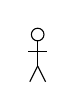
\begin{tikzpicture}[baseline=-0.4ex]
            \draw (0,0.25) circle (0.08);
            \draw (0,0.17)--(0,-0.15);
            \draw (-0.12,0.04)--(0.12,0.04);
            \draw (0,-0.15)--(-0.10,-0.35);
            \draw (0,-0.15)--(0.10,-0.35);
        \end{tikzpicture}\textit{ biểu diễn cho 1 học sinh)}
        \end{center}

        Lập bảng tần số cho dữ liệu được biểu diễn trong biểu đồ tranh trên.

        \answerline
        \answerline

        \item Biểu đồ Hình 7.7 cho biết số ngày sử dụng phương tiện đến trường của bạn Mai trong tháng Chín. Lập bảng tần số cho dữ liệu được biểu diễn trên biểu đồ.

        \begin{center}
        \begin{tikzpicture}[x=2cm,y=0.28cm]
            \foreach \y in {0,2,4,6,8,10,12,14,16} {
                \draw[base200] (0,\y)--(3.8,\y);
                \node[left] at (0,\y) {\y};
            }
            \draw[->] (0,0)--(4,0);
            \draw[->] (0,0)--(0,17);
            \foreach \x/\lab in {0.7/Xe buýt,1.9/Xe máy,3.1/Xe đạp} {
                \node[below,align=center] at (\x,0) {\lab};
            }
            \foreach \x/\h in {0.7/9,1.9/5,3.1/8} {
                \fill[base700] (\x-0.25,0) rectangle (\x+0.25,\h);
                \node[above] at (\x,\h) {\h};
            }
            \node[font=\bfseries] at (1.9,19) {Phương tiện đến trường của Mai};
            \node[below] at (1.9,-2.4) {Phương tiện đến trường};
            \node[rotate=90] at (-0.75,8.5) {Số ngày};
        \end{tikzpicture}

        \textit{Hình 7.7}
        \end{center}

        \answerline
        \answerline

        \item Người ta thống kê các loại ô tô chạy qua một trạm thu phí trong 1 giờ và vẽ được biểu đồ tần số như Hình 7.8.

        \begin{center}
        \begin{tikzpicture}[x=1.9cm,y=0.28cm]
            \foreach \y in {0,5,10,15} {
                \draw[base200] (0,\y)--(4.8,\y);
                \node[left] at (0,\y) {\y};
            }
            \draw[->] (0,0)--(5,0);
            \draw[->] (0,0)--(0,16);
            \foreach \x/\lab in {0.6/{Xe\\4 chỗ},1.7/{Xe\\7 chỗ},2.8/{Xe\\9 chỗ},4.0/{Xe 16 chỗ\\trở lên}} {
                \node[below,align=center] at (\x,0) {\lab};
            }
            \draw[base700,thick] (0.6,9)--(1.7,14)--(2.8,5)--(4.0,3);
            \foreach \x/\h in {0.6/9,1.7/14,2.8/5,4.0/3} {
                \fill[base700] (\x,\h) circle (2pt);
                \node[above right] at (\x,\h) {\h};
            }
            \node[font=\bfseries] at (2.4,18) {Số lượng các loại ô tô};
            \node[below] at (2.4,-4.1) {Loại xe};
            \node[rotate=90] at (-0.8,8) {Số xe};
        \end{tikzpicture}

        \textit{Hình 7.8}
        \end{center}

        \begin{questions}
            \item Lập bảng tần số cho dữ liệu được biểu diễn trên biểu đồ.

            \answerline
            \answerline

            \item Từ bảng tần số, hãy cho biết loại xe nào đi qua trạm thu phí nhiều nhất.

            \answerline
        \end{questions}

        \item Bảng thống kê sau cho biết số lượng các thiên tai xảy ra tại Việt Nam giai đoạn 1990 -- 2021.

        \begin{center}
        \begin{tblr}{
            colspec={Q[l] *{5}{Q[c]}},
            row{1}={font=\bfseries}
        }
            Loại thiên tai & Hạn hán & Bệnh dịch & Lũ lụt & Sạt lở đất & Bão \\
            Số lượng & 6 & 9 & 71 & 6 & 94 \\
        \end{tblr}
        \end{center}

        \begin{flushright}
            \textit{(Theo vietnam.opendevelopmentmekong.net)}
        \end{flushright}

        Vẽ biểu đồ tần số dạng cột và biểu đồ tần số dạng đoạn thẳng biểu diễn bảng thống kê trên.

        \answerline
        \answerline
        \answerline
    \end{questions}
\end{exercises}

\begin{practice}
    \subsection{Luyện tập}

    \begin{questions}[series=SBT]
        \item Tính đến hết SEA Games 32 đã có năm quốc gia từng lên ngôi vô địch bóng đá nam SEA Games, cụ thể như sau:

        \begin{center}
        \begin{tblr}{
            width=\linewidth,
            colspec={Q[l,3cm] X[l]},
            row{1}={font=\bfseries, halign=c},
            cells={valign=m}
        }
            Đội tuyển & Năm vô địch \\
            Thái Lan & 1975, 1981, 1983, 1985, 1993, 1995, 1997, 1999, 2001, 2003, 2005, 2007, 2013, 2015, 2017 \\
            Malaysia & 1961, 1977, 1979, 1989, 2009, 2011 \\
            Myanmar & 1965, 1967, 1969, 1971, 1973 \\
            Việt Nam & 1959; 2019, 2021 \\
            Indonesia & 1987, 1991, 2023 \\
        \end{tblr}
        \end{center}

        \begin{flushright}
            \textit{(Theo sportingnews.com)}
        \end{flushright}

        \begin{questions}
            \item Lập bảng tần số biểu diễn số lần vô địch môn bóng đá nam SEA Games của các quốc gia trên.

            \answerline
            \answerline

            \item Từ bảng tần số thu được ở câu a, hãy cho biết quốc gia nào vô địch môn Bóng đá nam SEA Games nhiều nhất, với mấy lần vô địch.

            \answerline
        \end{questions}

        \item Giáo viên dạy Toán ghi lại số bài tập mỗi học sinh trong lớp đã làm sau bài học tuần trước cho kết quả như sau:

        \[
        \begin{aligned}
            &4,\ 2,\ 0,\ 5,\ 4,\ 3,\ 2,\ 1,\ 3,\ 3,\ 6,\ 1,\ 3,\ 2,\ 4,\ 3,\ 5,\ 3,\\
            &3,\ 1,\ 4,\ 6,\ 1,\ 2,\ 3,\ 5,\ 3,\ 2,\ 4,\ 3,\ 1,\ 4,\ 4,\ 5,\ 6,\ 2.
        \end{aligned}
        \]

        \begin{questions}
            \item Lập bảng tần số cho dãy số liệu trên.

            \answerline
            \answerline

            \item Có bao nhiêu bạn trong lớp làm ít nhất ba bài tập?

            \answerline
        \end{questions}

        \item Bảng sau cho biết kết quả bình chọn môn thể thao được yêu thích nhất của các bạn học sinh lớp 9A (mỗi gạch biểu diễn cho một bạn bình chọn):

        \begin{center}
        \begin{tblr}{
            colspec={Q[l,3cm] Q[l,7cm]},
            cells={valign=m}
        }
            Bóng đá & {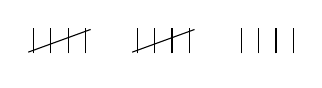
\begin{tikzpicture}[x=0.22cm,y=0.32cm,baseline=-0.5ex]
                \foreach \s in {0,1} {
                    \foreach \x in {0,1,2,3} \draw (\s*6+\x,0)--(\s*6+\x,1);
                    \draw (\s*6-0.3,0.05)--(\s*6+3.3,0.95);
                }
                \foreach \x in {12,13,14,15} \draw (\x,0)--(\x,1);
            \end{tikzpicture}} \\
            Cầu lông & {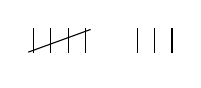
\begin{tikzpicture}[x=0.22cm,y=0.32cm,baseline=-0.5ex]
                \foreach \x in {0,1,2,3} \draw (\x,0)--(\x,1);
                \draw (-0.3,0.05)--(3.3,0.95);
                \foreach \x in {6,7,8} \draw (\x,0)--(\x,1);
            \end{tikzpicture}} \\
            Bóng bàn & {\begin{tikzpicture}[x=0.22cm,y=0.32cm,baseline=-0.5ex]
                \foreach \x in {0,1,2,3} \draw (\x,0)--(\x,1);
            \end{tikzpicture}} \\
            Môn khác & {\begin{tikzpicture}[x=0.22cm,y=0.32cm,baseline=-0.5ex]
                \foreach \x in {0,1,2,3} \draw (\x,0)--(\x,1);
                \draw (-0.3,0.05)--(3.3,0.95);
                \foreach \x in {6,7} \draw (\x,0)--(\x,1);
            \end{tikzpicture}} \\
        \end{tblr}
        \end{center}

        \begin{questions}
            \item Lập bảng tần số cho kết quả bình chọn trên.

            \answerline
            \answerline

            \item Dựa vào bảng tần số thu được ở câu a, cho biết môn thể thao nào được các bạn yêu thích nhất.

            \answerline
        \end{questions}

        \item Biểu đồ sau cho biết kết quả khảo sát trình độ tiếng Anh của sinh viên cuối năm thứ nhất ở một trường đại học:

        \begin{center}
        \begin{tikzpicture}[x=1.35cm,y=0.024cm]
            \foreach \y in {0,50,100,150,200,250,300,350,400} {
                \draw[base200] (0,\y)--(6,\y);
                \node[left] at (0,\y) {\y};
            }
            \draw[->] (0,0)--(6.2,0);
            \draw[->] (0,0)--(0,420);
            \foreach \x/\lab in {0.7/A1,1.8/A2,2.9/B1,4.0/B2,5.1/C1} {
                \node[below] at (\x,0) {\lab};
            }
            \foreach \x/\h in {0.7/102,1.8/115,2.9/345,4.0/35,5.1/3} {
                \fill[base700] (\x-0.23,0) rectangle (\x+0.23,\h);
                \node[above] at (\x,\h) {\h};
            }
            \node[font=\bfseries,align=center] at (3,470) {Kết quả khảo sát trình độ tiếng Anh của sinh viên\\cuối năm thứ nhất};
            \node[below] at (3,-55) {Trình độ tiếng Anh};
            \node[rotate=90] at (-0.85,210) {Số sinh viên};
        \end{tikzpicture}
        \end{center}

        \begin{questions}
            \item Đọc và giải thích số liệu được biểu diễn trên hai cột bất kì của biểu đồ.

            \answerline

            \item Lập bảng tần số cho dữ liệu được biểu diễn trên biểu đồ.

            \answerline
            \answerline

            \item Để tốt nghiệp đại học, sinh viên cần có trình độ tiếng Anh ở mức B1 trở lên. Ước lượng tỉ lệ sinh viên cuối năm thứ nhất đã đạt chuẩn trình độ tiếng Anh.

            \answerline
            \answerline
        \end{questions}

        \item Số $\pi$ với 50 chữ số sau dấu phẩy thập phân như sau:

        \[
            3{,}141\ 592\ 653\ 589\ 793\ 238\ 462\ 643\ 383\ 279\ 502\ 884\ 197\ 169\ 399\ 375\ 10.
        \]

        \begin{questions}
            \item Lập bảng tần số cho các chữ số từ 0 đến 9 xuất hiện sau dấu phẩy thập phân.

            \answerline
            \answerline

            \item Chữ số nào xuất hiện nhiều nhất, ít nhất?

            \answerline
        \end{questions}

        \item Cho biểu đồ tần số dạng đoạn thẳng sau:

        \begin{center}
        \begin{tikzpicture}[x=1.25cm,y=0.45cm]
            \foreach \y in {0,2,4,6,8,10,12,14} {
                \draw[base200] (0,\y)--(7,\y);
                \node[left] at (0,\y) {\y};
            }
            \draw[->] (0,0)--(7.2,0);
            \draw[->] (0,0)--(0,15);
            \foreach \x/\lab in {1/5,2/6,3/7,4/8,5/9,6/10} {
                \node[below] at (\x,0) {\lab};
            }
            \draw[base700,thick] (1,2)--(2,6)--(3,10)--(4,13)--(5,7)--(6,1);
            \foreach \x/\h in {1/2,2/6,3/10,4/13,5/7,6/1} {
                \draw[fill=white] (\x,\h) circle (2.5pt);
                \node[above right] at (\x,\h) {\h};
            }
            \node[font=\bfseries] at (3.5,16.5) {Kết quả kiểm tra môn Toán};
            \node[below] at (3.5,-1.5) {Điểm};
            \node[rotate=90] at (-0.85,7.5) {Số học sinh};
        \end{tikzpicture}
        \end{center}

        \begin{questions}
            \item Lập bảng tần số cho dữ liệu được biểu diễn trên biểu đồ.

            \answerline
            \answerline

            \item Điểm nào có nhiều học sinh đạt nhất?

            \answerline
        \end{questions}

        \item Một túi chứa một số viên bi có cùng kích thước, mỗi viên bi có một trong các màu đen, trắng, đỏ, vàng. Thực hiện lấy bi 20 lần, mỗi lần lấy một viên xem viên bi có màu gì sau đó trả bi lại túi, trộn đều. Kết quả trong 20 lần lấy bi có 8 lần lấy được bi đen, 4 lần lấy được bi đỏ, 6 lần lấy được bi trắng, 2 lần lấy được bi vàng.

        \begin{questions}
            \item Lập bảng tần số cho kết quả thu được.

            \answerline
            \answerline

            \item Vẽ biểu đồ tần số dạng cột biểu diễn bảng tần số thu được ở câu a.

            \answerline
            \answerline
            \answerline
        \end{questions}

        \item Thống kê số ngày nằm viện của 20 bệnh nhân được kết quả như sau:

        \[
            5,\ 7,\ 4,\ 6,\ 8,\ 10,\ 6,\ 7,\ 8,\ 8,\ 6,\ 5,\ 8,\ 5,\ 4,\ 6,\ 5,\ 7,\ 4,\ 6.
        \]

        \begin{questions}
            \item Lập bảng tần số cho dãy số liệu trên.

            \answerline
            \answerline

            \item Vẽ biểu đồ tần số dạng đoạn thẳng biểu diễn bảng tần số thu được ở câu a.

            \answerline
            \answerline
            \answerline
        \end{questions}
    \end{questions}
\end{practice}

